\documentclass[10pt]{beamer}

\usetheme{metropolis}
\usepackage{appendixnumberbeamer}

\usepackage{booktabs}
\usepackage[scale=2]{ccicons}
\usepackage{graphicx}
\usepackage{hyperref}
\usepackage{circuitikz}
\usepackage{pdflscape}
\usepackage{smartdiagram}

\usepackage{color}
\usepackage{listings}

\lstset{
	basicstyle=\footnotesize\ttfamily,
    keepspaces=true,
    showstringspaces=false,
    language=PHP,
    commentstyle=\ttfamily,
}

\usepackage[OT4]{polski}
\usepackage[utf8]{inputenc}

\usepackage{pgfplots}
\usepgfplotslibrary{dateplot}

\usepackage{xspace}
\newcommand{\themename}{\textbf{\textsc{metropolis}}\xspace}

\setbeamertemplate{frame footer}{}
\setbeamertemplate{frame numbering}{}

\usetikzlibrary{shapes,arrows}

\tikzstyle{decision} = [diamond, draw, fill=blue!20, 
    text width=4.5em, text badly centered, node distance=3cm, inner sep=0pt]
\tikzstyle{block} = [rectangle, draw, fill=blue!20, 
    text width=5em, text centered, rounded corners, minimum height=4em]
\tikzstyle{line} = [draw, -latex']
\tikzstyle{cloud} = [draw, ellipse,fill=red!20, node distance=3cm,
    minimum height=2em]


\title{Implementacja logiki biznesowej}

\subtitle{Zaawansowane metody programowania}
\author{mgr inż. Krzysztof Rewak}
\date{\today}
\institute{Wydział Nauk Technicznych i Ekonomicznych \\ Państwowa Wyższa Szkoła Zawodowa im. Witelona w Legnicy}

\begin{document}

\maketitle

\begin{frame}{Plan prezentacji}
  \setbeamertemplate{section in toc}[sections numbered]
  \tableofcontents[hideallsubsections]
\end{frame}


\section{Logika biznesowa}

\begin{frame}{Logika}
	Według SJP \textbf{logika} to nauka zajmująca się znajdowaniem praw rządzących ludzkim rozumowaniem, a także wnioskowaniem.
\end{frame}

\begin{frame}{Proces biznesowy}
	\textbf{Procesem biznesowym} jest natomiast seria zadań, których wykonanie w odpowiedniej kolejności doprowadzi do zrealizowania celu.
\end{frame}

\begin{frame}{Logika biznesowa}
	Wynikiem syntezy tych dwóch pojęć może być \textbf{logika biznesowa}.
	
	Upraszczając, jest to sposób przeniesienia procesów biznesowych do programu komputerowego, ale zachowując wszystkie reguły domeny.
\end{frame}

\begin{frame}{Domena}
	Domeną nazywamy dziedzinę, w której przestrzeni będzie funkcjonowało nasze oprogramowanie.
	
	System, który będzie wykorzystywany przez księgową małego przedsiębiorstwa, powinien implementować zasady rządzące księgowością małego przedsiębiorstwa. Trzeba mieć świadomość, że każda domena, choćby z wierzchu do siebie podobna, jest inna od pozostałych. 
\end{frame}

\begin{frame}[fragile]{Domena}
	
	\ \\
	
	Obliczanie podatku od dochodu mogłoby wydawać się proste, ale wszystko zależy od poznania domeny.
	
	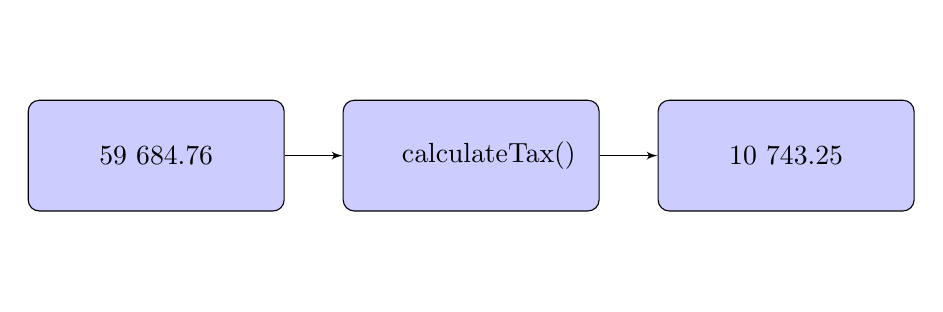
\begin{tikzpicture}[node distance=4cm, minimum size=3.25cm]
		\node [block] (in) {59 684.76};
		\node [block, right of=in] (calc) {calculateTax()};
		\node [block, right of=calc] (out) {10 743.25};
		
		\path [line] (in) -- node {} (calc);
		\path [line] (calc) -- node {} (out);
	\end{tikzpicture}
	
	Jeżeli nasza wiedza kończy się na powyższym wykresie, szybko można założyć, że funkcja obliczająca wygląda następująco:
	
	\ \\
	
	\begin{lstlisting}
func calculateTax(income double) double {
  return income * 18 / 100;
}
	\end{lstlisting}
\end{frame}

\begin{frame}{Domena}
	Wszystko okej, ale co w przypadku...
	\begin{itemize}
	\item przekroczenia produ podatkowego?
	\item rozliczania się z małżonkiem?
	\item rozliczania się w innym państwie?
	\item dziesiątek innych przypadków?
	\end{itemize}
\end{frame}

\begin{frame}{Domena}
	Jednym z najczęstszych źródeł problemów przy programowaniu systemów internetowych (ale nie tylko!) jest brak zrozumienia domeny i procesów biznesowych, które mają zostać ujęte w tymże systemie.
\end{frame}

\begin{frame}{Domena}
	Dobrze zamodelowany i zaprojektowany proces to często ponad połowa wykonanej pracy.
\end{frame}

\begin{frame}{Modelowanie domeny}
	Jak poprawnie zamodelować proces biznesowy?
	\begin{itemize}
		\item na kartce i z ołówkiem lub na tablicy i z mazakiem,
		\item korzystając z bardziej wyrafinowanych metod takich jak \emph{event storming},
		\item lub w dowolny inny zrozumiały dla programistów sposób.
	\end{itemize}
	
	Często może się okazać, że dwóch profesjonalistów stworzy dwa różne modele tego samego procesu biznesowego. Czy to źle? Skądże!
\end{frame}

\section{Narzędzia}

\begin{frame}{Jak zaimplementować logikę biznesową?}
	Każdy problem wymaga indywidualnego podejścia. Czy to oznacza, że mamy wynajdować koło na nowo?
\end{frame}

\begin{frame}[fragile]{MVC?}

	\ \\
	
	\hspace*{1.25cm}%
	\begin{tikzpicture}[node distance=4cm, minimum size=2cm, auto]
	
		\node [circle, fill=orange,inner sep=3pt] (user) {użytkownik};
		
		\node [block, above right of=user] (controller) {kontroler};
		\node [block, above left of=user] (view) {widok};
		\node [block, above left of=controller] (model) {model};
		
	
		\path [line] (user) -- node[label={[shift={(2,-3.5)}]wywołuje}] {} (controller);
		\path [line] (controller) -- node[label={[shift={(2,-0.5)}]żąda zmian}] {} (model);
		\path [line] (model) -- node[label={[shift={(-2,-0.5)}]uaktualnia}]  {} (view);
		\path [line] (view) -- node[label={[shift={(-2,-3.5)}]wyświetla}] {} (user);
	\end{tikzpicture}
\end{frame}

\begin{frame}[fragile]{A może MRVRMCES?}
	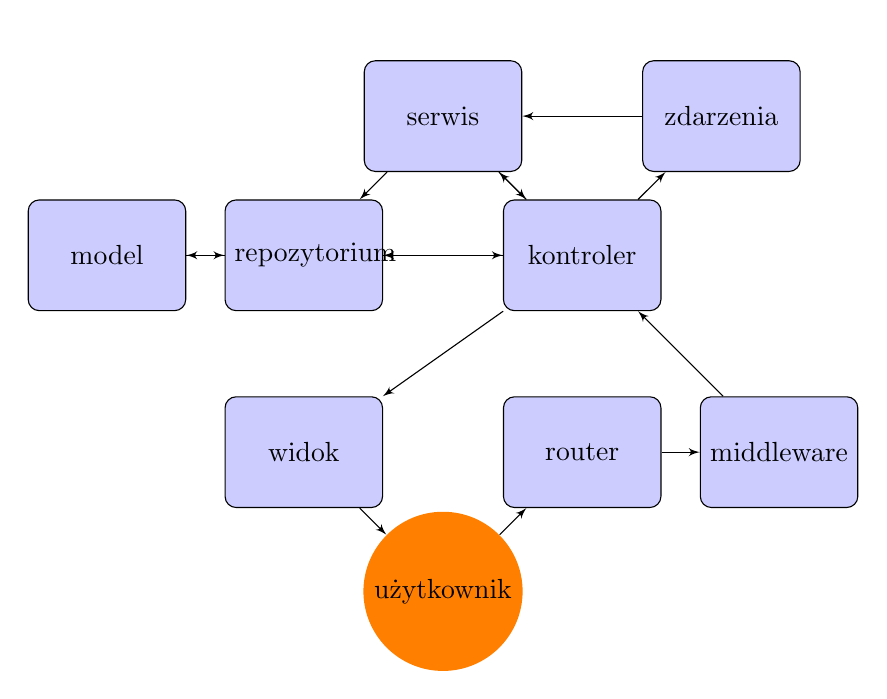
\begin{tikzpicture}[node distance=2.5cm, minimum size=2cm, auto]
	
		\node [circle, fill=orange,inner sep=3pt] (user) {użytkownik};
		
		\node [block, above right of=user] (router) {router};
		\node [block, above left of=user] (view) {widok};
		\node [block, right of=router] (middleware) {middleware};
		
		\node [block, above of=router] (controller) {kontroler};
		\node [block, above of=view] (repo) {repozytorium};
		\node [block, left of=repo] (model) {model};
		
		\node [block, above left of=controller] (service) {serwis};
		\node [block, above right of=controller] (event) {zdarzenia};
		
		\path [line] (user) -- node {} (router);
		\path [line] (router) -- node {} (middleware);
		\path [line] (middleware) -- node {} (controller);
		\path [line] (controller) -- node {} (service);
		\path [line] (controller) -- node {} (event);
		\path [line] (event) -- node {} (service);
		\path [line] (service) -- node {} (repo);
		\path [line] (controller) -- node {} (repo);
		\path [line] (repo) -- node {} (model);
		\path [line] (controller) -- node {} (view);
		\path [line] (view) -- node {} (user);
		
		\path [line] (service) -- node {} (controller);
		\path [line] (repo) -- node {} (controller);
		\path [line] (model) -- node {} (repo);
	\end{tikzpicture}
\end{frame}

\section{Serwisy}

\begin{frame}{Serwisy}
	Spójrzmy na przykładowy kontroler \texttt{ArticleController}:
\end{frame}

\begin{frame}[fragile]{Serwisy}
	\begin{lstlisting}
class ArticleController (Controller)

  method updateArticle(Id: Int, Request: Request): Void
    @Article := Article::Get(Id)
    foreach @Tag in @Article.Tags
      if Array.in(@Tag.Id, Request.Get("tags"))
        if not @Tag.Selected
          @Article.Delete(@Tag)
        endif
      else
        if @Tag.Selected
          @Article.Add(@Tag)
        endif
      endif
    endforeach
    if @Article.Update(Request.Except("tags"))
      Mail(@Article.User.Email, "Article has been changed.")
    endif
  endmethod
  
endclass
	\end{lstlisting}
\end{frame}

\begin{frame}[fragile]{Serwisy}

	\ \\
	
	Może lepiej go nieco skrócić i przerzucić część logiki do innych klas?

	\begin{lstlisting}
class ArticleController (Controller)

  method updateArticle(Id: Int, Request: Request): void
    @Article := Article::Get(Id)

    @ArticleTagManager = new ArticleTagManager
    @ArticleTagManager.ManageTags(@Article, Request.Get("tags"))

    if @Article.Update(Request.Except("tags"))
      @MailService = new MailService
      @MailService.SetReceiver(@Article.User)
      @MailService.SetMessasge("Article has been changed.")
      @MailService.Send()
    endif
  endmethod

endclass
	\end{lstlisting}
\end{frame}

\begin{frame}{Serwisy}
	Serwis służy przede wszystkim do odseparowania logiki.
\end{frame}

\begin{frame}{Serwisy}
	Dzięki wykorzystaniu serwisów można:
	\begin{itemize}
		\item zmniejszyć niepotrzebną redundancję w kodzie,
		\item wykorzystać tę samą funkcjonalność w wielu miejscach,
		\item realizować zasadę pojedynczej odpowiedzialności,
		\item wygodnie testować aplikację.
	\end{itemize}
\end{frame}

\begin{frame}{Testowanie serwisów}
	O ileż łatwiej jest wywołać w teście klasę pojedynczego serwisu z konkretnymi danymi niż przebijać się przez cały kontroler i budować chociażby skomplikowane parametry z zapytania serwera?
\end{frame}

\begin{frame}[fragile]{Testowanie serwisów}
	\begin{lstlisting}
class PromoteUserToAdminService implements UserServiceInterface {

  protected $user;
  protected $grantor;

  public function setUser(User $user): self {
    $this->user = $user;
    return $this;
  }

  public function setGrantor(User $grantor): self {
    $this->grantor = $grantor;
    return $this;
  }

  public function run(): bool {
    $this->user->role = User::ADMIN;
    Log::info(/* message */);
    return $this->user->save();
  }

}
	\end{lstlisting}
\end{frame}

\begin{frame}[fragile]{Testowanie serwisów}
	\begin{lstlisting}
class ExampleTest extends TestCase {

  public function userPromotionTest(): void {
    $user = User::create(["login" => "jsmith"]);
    $grantor = User::create([
      "login" => "admin",
      "role" => User::ADMIN,
     ]);
    
    $service = new PromoteUserToAdminService();
    $service->setUser($user);
    $service->setGrantor($grantor);
      
    $this->assertTrue($service->run());
  }
  
}
	\end{lstlisting}
\end{frame}

\section{Repozytoria}

\begin{frame}{Repozytoria}
	\textbf{Repozytorium} służy do oddzielenia logiki biznesowej od warstwy modelowania i mapowania danych.
\end{frame}

\begin{frame}[fragile]{Repozytoria}
	Ideą stojącą za repozytoriami jest potrzeba ujednolicenia przetwarzania danych.
\end{frame}

\begin{frame}[fragile]{Repozytoria}	
	Wyobraźmy sobie kontroler wypisujący wszystkie produkty w sklepie internetowym. Czy z poziomu kontrolera powinniśmy wywoływać połączenie do bazy danych, pobierać zmapowane na modele informacje i przekazać dalej do widoku? A co w przypadku, gdy dane czasami będą pobierane z cache'a? Albo z pliku? Albo z jeszcze innego miejsca?
\end{frame}

\begin{frame}[fragile]{Repozytoria}
	\begin{lstlisting}
public interface Repository<T> {
    void create(T item);
    void update(T item);
    void delete(T item);
    List<T> get();
    T get(int id)
}
	\end{lstlisting}
\end{frame}

\begin{frame}{Repozytoria}
	Repozytorium można oczywiście dostosować do własnych potrzeb, ale należy uważać, aby nie przekombinować!
	
	Tzw. \emph{overengineering} może doprowadzić do wielu problemów z zaciemnieniem kodu na czele.
\end{frame}

\section{Wstrzykiwanie zależności}

\begin{frame}{Wstrzykiwanie zależności}
	Repozytoria i serwisy są wygodnymi narzędziami, jednak dodanie każdego nowego komponentu wymaga utworzenia bezpośrednich zależności między klasami. Okazuje się, że nie zawsze jest to dobrym rozwiązaniem.
\end{frame}

\begin{frame}{Wstrzykiwanie zależności}
	Z pomocą może przyjść wzorzec projektowy wstrzykiwania zależności (ang. \emph{dependency injection}.
	
	Oto kontroler, którego metoda wyświetla wszystkich zarejestrowanych użytkowników:
\end{frame}

\begin{frame}[fragile]{Wstrzykiwanie zależności}
	\begin{lstlisting}
	
	
public class UsersController : Controller
{

  public ActionResult All()
  {
    UserRepository repository = new UserRepository();
    var users = repository.ListAll();

    return View(users);
  }
  
}
	\end{lstlisting}
\end{frame}

\begin{frame}[fragile]{Wstrzykiwanie zależności}
	\begin{lstlisting}
	
	
public class UsersController : Controller
{
  
  private readonly IUserRepository _repository;

  public UsersController(IUserRepository repository)
  {
    _repository = repository;
  }

  public ActionResult All()
  {
    var users = _repository.ListAll();
    return View(users);
  }

}
	\end{lstlisting}
\end{frame}

\begin{frame}{Wstrzykiwanie zależności}
	Obiekty są w takim wypadku przekazywane jako już utworzone instancje, przez co architektura całej aplikacji jest bardziej elastyczna i modułowa.
	
	Wstrzyknąć można - w zależności od języka - obiekt według klasy, klasy po dziedziczeniu lub po implementowanym interfejsie. Ta ostatnia metoda jest szczególnie warta wspomnienia, gdyż umożliwia pełne wykorzystanie wstrzykiwania zależności.
\end{frame}

\begin{frame}[fragile]{Wstrzykiwanie zależności}
	Skąd aplikacja wie, co ma wstrzyknąć do której klasy? Można zarejestrować konkretne połączenia w odpowiednim miejscu:

	\begin{lstlisting}
public void ConfigureServices(IServiceCollection services)
{
  // (...)
  services.AddScoped<IUserRepository, UserRepository>();
}
	\end{lstlisting}

	Ale część frameworków (Laravel, Symfony) pozwalają na tzw. \emph{auto-wiring} i automatyczne wstrzykiwanie zależności na podstawie przestrzeni nazw i nazw klas.
\end{frame}

\begin{frame}{Wstrzykiwanie zależności}
	DI pozwala na wygodne testowanie aplikacji.
	
	Wyobraźmy sobie, że mamy repozytorium, które musi się podłączyć do bazy danych, pobrać rekordy, przetworzyć je i przekazać do testowanej przez nas klasy. Jeżeli testujemy inną funkcjonalność niż samo pobranie, możemy utworzyć tzw. \emph{mock}, czyli zaślepkę z odpowiednio spreparowanymi danymi na czas testów.
\end{frame}

\section{Zdarzenia}

\begin{frame}{Zdarzenia}
	Wiele nowoczesnych frameworków webowych pozwala na wykorzystywanie zdarzeń (\emph{eventów}) lub sygnałów (\emph{signals}). 
	
	Zdarzenie to proste powiadomienie o tym, że coś się ma wydarzyć. Odpowiedni nasłuchujący \emph{listener} powinien takie zdarzenie odebrać, przetworzyć i uruchomić odpowiednie procedury.
\end{frame}

\begin{frame}[fragile]{Zdarzenia}
	Wysłanie sygnału może wyglądać tak:

	\begin{lstlisting}
class CartController:

  # (...)
  
  def finish_order(self):
    # (...)
    place_order.send(sender=self.__class__, cart=self.cart)
	\end{lstlisting}
	
	... a odebranie następująco:
	
	\begin{lstlisting}
def place_order(sender, **kwargs):
  order = Order.objects.create()
  order.timestamp = datetime.datetime.now()
  # (...)
	\end{lstlisting}
\end{frame}

\begin{frame}{Zdarzenia}
	Oczywiście nic nie stoi na przeszkodzie, aby przy realizacji wydarzenia wykorzystać na przykład uprzednio zaprojektowany serwis lub pobrać dane z repozytorium.
\end{frame}

\begin{frame}{Zdarzenia}
	Ponadto część frameworków oferuje wbudowane zdarzenia dla operacji na swoich modelach.
	
	Przykładowo Laravel operuje na zdarzeniach: \texttt{retrieved}, \texttt{creating}, \texttt{created}, \texttt{updating}, \texttt{updated}, \texttt{saving}, \texttt{saved}, \texttt{deleting}, \texttt{deleted}, \texttt{restoring}, \texttt{restored}.
	
	Django: \texttt{pre\_save}, \texttt{post\_save}, \texttt{pre\_delete}, \texttt{post\_delete}, \texttt{m2m\_changed}.
	
	Wszystko powinno być jasno opisane w dokumentacji wybranego frameworka.
\end{frame}

\begin{frame}[fragile]{Zdarzenia}
	\begin{lstlisting}
class CourseGroupClass extends \Phalcon\Mvc\Model {

  // (...)

  public function afterCreate() {
    $students = $this->group->groupStudents;
    foreach($students as $student) {
      $grade = new Grade();
      $grade->save([
        "course_group_student_id" => $student->id,
        "course_group_class_id" => $this->id,
      ]);
    }
  }
  
}

	\end{lstlisting}
\end{frame}

\section{Podsumowanie}

\begin{frame}{Bibliografia i ciekawe źródła}
  
	\begin{thebibliography}{9}
		
		\bibitem{service}
		\url{https://javastart.pl/static/programowanie-android/services/}
		
		\bibitem{repo}
		\url{http://designpatternsphp.readthedocs.io/pl/latest/More/Repository/README.html}
		
		\bibitem{di}
		\url{http://designpatternsphp.readthedocs.io/pl/latest/Structural/DependencyInjection/README.html}
		
	\end{thebibliography}

\end{frame}

\appendix

\begin{frame}[standout]
	Pytania?
\end{frame}

\begin{frame}{}

	Kod prezentacji dostępny jest w repozytorium git pod adresem \texttt{https://bitbucket.org/krewak/pwsz-zmp} \\ \ \\

	\begin{figure}
		\centering
		\href{https://bitbucket.org/krewak/pwsz-ppsi}{
			\includegraphics[width=.15\textwidth]{../_template/bitbucket.png}
		}
	\end{figure}
	
	Wszystkie informacje dot. kursu dostępne są pod adresem \texttt{http://pwsz.rewak.pl/kursy/10} \\ \ \\

	\begin{figure}
		\centering
		\href{http://pwsz.rewak.pl/kursy/3}{
			\includegraphics[width=.15\textwidth]{../_template/rewak.png}
		}
	\end{figure}

\end{frame}

\end{document}
